\chapter{Method Description and Implementation}
\label{ch:method}

This chapter discusses the implementation and solution of the LDO equations in Denovo,
the parallel discrete ordinates radiation transport code package in the Exnihilo code 
suite \cite{exum}. First, a comparison of the traditional formulation of the discrete 
ordinates equations with the LDO equations is presented to demonstrate the difference 
in implementing the two separate sets of equations. Then, a brief discussion of 
scattering is given to highlight the specific differences between the two sets of 
equations with respect to how scattering is handled from the perspective of 
implementation. Following that is an overview of the quadrature sets used in solving 
the LDO equations in Denovo. Finally, we list
and discuss the restrictions of using the LDO equations in combination with Exnihilo 
and ADVANTG for the purpose of Monte Carlo variance reduction parameter generation.

\section{Operator Form}
\subsection{Traditional Discrete Ordinates Formulation}

When considering deterministic methods, it is often instructive to think about the NTE 
in operator form. In accordance with the discretization in Section \ref{sec:disc}, the 
operator form of the traditional discrete ordinates equations \cite{exmm} is

\begin{align}
\ve{L}\Psi &= \ve{MS}\Phi + Q, \\
\Phi &= \ve{D}\Psi\: \text{ where } \ve{D} = \ve{M}^\top\ve{W}, \\
\left(\ve{I} - \ve{DL}^{-1}\ve{MS}\right)\Phi &= \ve{DL}^{-1}Q.
\label{l_inv}
\end{align}

\noindent The operators will be defined below, with the exception of $\ve{L}$, the
transport operator. When solving Equation \ref{l_inv}, the operation $\ve{L}^{-1}$ is
referred to as a ``sweep''; $\ve{L}$ is implicitly formed as a lower-left triangular
matrix and is inverted by ``sweeping'' through the spatial mesh in the direction of
particle flow \cite{exmm}.
With this formulation, at each spatial unknown, with energy groups defined over the 
range $g\in[0,G-1]$ as described previously, we can write

\begin{align}
    \ve{L}
    &\begin{pmatrix}
      \Psi_0 \\
      \Psi_1 \\
      \vdots   \\
      \Psi_{G-1}  \nonumber
    \end{pmatrix} = \\
    &\qquad\begin{pmatrix}
      [\ve{M}] & 0 & 0 & 0 \\
      0 & [\ve{M}] & 0 & 0 \\
      0 & 0 & \ddots & \vdots \\
      0 & 0 & \cdots & [\ve{M}] \\
    \end{pmatrix}
    %%
    \begin{pmatrix}
      [\ve{S}]_{0\sa0} & [\ve{S}]_{1\sa0} & \cdots & [\ve{S}]_{G-1\sa0} \\
      [\ve{S}]_{0\sa1} & [\ve{S}]_{1\sa1} & \cdots & [\ve{S}]_{G-1\sa1} \\
      \vdots & \vdots & \ddots & \vdots \\
      [\ve{S}]_{0\sa G-1} & [\ve{S}]_{1\sa G-1} & \cdots & [\ve{S}]_{G-1\sa G-1}
    \end{pmatrix}
    \begin{pmatrix}
      \Phi_0 \\
      \Phi_1 \\
      \vdots   \\
      \Phi_{G-1}
    \end{pmatrix}
    %%
    \\&\fq\fq\fq\qquad\qquad\qquad+
    \begin{pmatrix}
      Q_0 \\
      Q_1 \\
      \vdots  \\
      Q_{G-1}
    \end{pmatrix}, \nonumber
    \label{eq:matrix-transport}
\end{align}

\noindent where the notation $[\cdot]_g$ indicates a block matrix over all
unknowns for a single group.  

Here, the angular flux vector for group $g$ over angles $1,\ldots,N$ is defined as

\begin{equation}
  \Psi_g = \begin{pmatrix}
    \psi^g_1 & \psi^g_2 & \psi^g_3 & \cdots \psi^g_N
  \end{pmatrix}^\top,
\label{psiv}
\end{equation}

\noindent with the external source vector $Q_g$
defined similarly. The operator $\ve{M}$ is the ``moment-to-discrete'' matrix and is 
used to project harmonic moments onto discrete angle space. It is defined as

\begin{equation}
[\ve{M}] = \begin{pmatrix}
\Ye{00}{1} & \Ye{10}{1} & \Yo{11}{1} & \Ye{11}{1} & \cdots & \Yo{PP}{1} & \Ye{PP}{1} \\
\Ye{00}{2} & \Ye{10}{2} & \Yo{11}{2} & \Ye{11}{2} & \cdots & \Yo{PP}{2} & \Ye{PP}{2} \\
\Ye{00}{3} & \Ye{10}{3} & \Yo{11}{3} & \Ye{11}{3} & \cdots & \Yo{PP}{3} & \Ye{PP}{3} \\
\vdots     & \vdots     & \vdots     & \vdots     & \ddots & \vdots     & \vdots     \\
\Ye{00}{N} & \Ye{10}{N} & \Yo{11}{N} & \Ye{11}{N} & \cdots & \Yo{PP}{N} & \Ye{PP}{N}
  \end{pmatrix}\:.
\label{mtod}
\end{equation}

\noindent Note that $[\ve{M}]$ is dependent only on angle and is therefore the same for
each energy group. The operator $\ve{D}$ is the ``discrete-to-moment'' matrix; it is
used to calculate the moments of the angular flux from discrete angular flux values. 
$\ve{D}$ is calculated as $\ve{M}^\top\ve{W}$, where $\ve{W}$ is a diagonal matrix of 
quadrature weights \cite{exmm}, and it is written as

\begin{equation}
  [\ve{D}] = \begin{pmatrix}
    w_1\Ye{00}{1} & w_2\Ye{00}{2} & w_3\Ye{00}{3} & \cdots & w_N\Ye{00}{N} \\ 
    w_1\Ye{10}{1} & w_2\Ye{10}{2} & w_3\Ye{10}{3} & \cdots & w_N\Ye{10}{N} \\
    w_1\Yo{11}{1} & w_2\Yo{11}{2} & w_3\Yo{11}{3} & \cdots & w_N\Yo{11}{N} \\
    w_1\Ye{11}{1} & w_2\Ye{11}{2} & w_3\Ye{11}{3} & \cdots & w_N\Ye{11}{N} \\
    \vdots        & \vdots        & \vdots        & \ddots & \vdots        \\
    w_1\Yo{PP}{1} & w_2\Yo{PP}{2} & w_3\Yo{PP}{3} & \cdots & w_N\Yo{PP}{N} \\
    w_1\Ye{PP}{1} & w_2\Ye{PP}{2} & w_3\Ye{PP}{3} & \cdots & w_N\Ye{PP}{N}
  \end{pmatrix}\:.
\end{equation}

\noindent Like $[\ve{M}]$, $[\ve{D}]$ is dependent only on angle and is the same for
each energy group. The scattering cross section matrices are defined as

\begin{equation}
  [\ve{S}]_{g'\rightarrow g} = \begin{pmatrix}
    \Sigg{0} & 0 & 0 & 0 & 0 & 0 & 0 \\
    0 & \Sigg{1} & 0 & 0 & 0 & 0 & 0 \\
    0 & 0 & \Sigg{1} & 0 & 0 & 0 & 0 \\
    0 & 0 & 0 & \Sigg{1} & 0 & 0 & 0 \\
    0 & 0 & 0 & 0 & \ddots   & 0 & 0 \\
    0 & 0 & 0 & 0 & 0 & \Sigg{P} & 0 \\
    0 & 0 & 0 & 0 & 0 & 0 & \Sigg{P}
  \end{pmatrix}\:,
\label{denovo_scatter}
\end{equation}

\noindent where these scattering cross section coefficient values come from data libraries based
on experimental measurements. Finally, the flux moment vectors are defined as

\begin{align}
  \Phi_g = \begin{pmatrix}
    \even_{00} & \even_{10} & \odd_{11} & \even_{11} & \even_{20}
    & \cdots & \odd_{PP} & \even_{PP}
  \end{pmatrix}^\top\:,
\end{align}

\noindent where the flux moments are evaluated as listed in 
Equation \ref{sph_harm_exp}. As we will describe below in Section \ref{sec:flux}, the 
goal of solving the discrete ordinates equations is to solve for these flux moments 
and then use
the flux moments to calculate the scalar flux. In summary, the traditional discrete 
ordinates discretizations are captured in the preceding matrices; they can be used to
analyze behavior and performance and can be compared against other discretizations.

\subsection{LDO Formulation}

As discussed in Chapter \ref{bgch}, although the LDO equations are formally the same
as the traditional discrete ordinates equations, there are several key differences
between the sets of equations. Here we present and discuss the operator form of
the LDO equations as a comparison to the operator form of the discrete ordinates 
equations shown above. The operator form of the LDO equations is

\begin{align}
\ve{L}\Psi &= \ve{\tilde{S}J}\Psi + Q, \\
\left(\ve{I} - \ve{L^{-1} \tilde{S}J}\right)\Psi &= \ve{L^{-1}}Q.
\end{align}

\noindent Letting $\ve{D} \equiv \ve{I}$ with 
$\ve{L^{-1}} = \ve{I}\ve{L^{-1}} = \ve{D}\ve{L^{-1}}$, we then have

\begin{equation}
\left(\ve{I} - \ve{D L^{-1} \tilde{S}J}\right)\Psi = \ve{D L^{-1}}Q.
\label{ldo_op}
\end{equation}

\noindent Equation \ref{ldo_op} is in the same form as Equation \ref{l_inv}, so we 
can apply the same solution techniques to both sets of equations.

In contrast to Equation \ref{l_inv}, however, Equation \ref{ldo_op} contains the 
Lagrange interpolation matrix $\ve{J}$ rather than the moment-to-discrete operator 
$\ve{M}$, and $\ve{\tilde{S}}$ contains the new formulation of scattering cross 
sections specific to the LDO equations. Additionally, when solving the LDO equations, 
we are solving for the angular flux coefficients rather than flux moments.
Now, at each spatial unknown, with energy groups 
again defined over the range $g\in[0,G-1]$, we have

\begin{align}
    \ve{L}
    &\begin{pmatrix}
      \Psi_0 \\
      \Psi_1 \\
      \vdots   \\
      \Psi_{G-1}  \nonumber
    \end{pmatrix} = \\
    &\qquad\begin{pmatrix}
      [\ve{\st}]_{0\sa 0}   & [\ve{\st}]_{1\sa0}    & \cdots & [\ve{\st}]_{G-1\sa0} \\
      [\ve{\st}]_{0\sa 1}   & [\ve{\st}]_{1\sa1}    & \cdots & [\ve{\st}]_{G-1\sa1} \\
      \vdots                & \vdots                & \ddots & \vdots               \\
      [\ve{\st}]_{0\sa G-1} & [\ve{\st}]_{1\sa G-1} & \cdots & [\ve{\st}]_{G-1 \sa G-1}
    \end{pmatrix}
    \begin{pmatrix}
      [\ve{J}] & 0 & 0 & 0 \\
      0 & [\ve{J}] & 0 & 0 \\
      0 & 0 & \ddots & \vdots \\
      0 & 0 & \cdots & [\ve{J}] \\
    \end{pmatrix}
    \begin{pmatrix}
      \Psi_0 \\
      \Psi_1 \\
      \vdots   \\
      \Psi_{G-1}
    \end{pmatrix}
    %%
    \\&\fq\fq\fq\qquad\qquad\quad+
    \begin{pmatrix}
      Q_0 \\
      Q_1 \\
      \vdots  \\
      Q_{G-1} \nonumber
    \end{pmatrix},
\end{align}

\noindent where the block matrix notation still holds. The angular flux coefficient 
vector and external source vector are formed as listed in Equation \ref{psiv}.
The operator [$\ve{J}$] performs the Lagrange interpolation. It is constructed as the
inverse of the Gram matrix, $\ve{G}$, which is calculated as

\begin{equation}
  \ve{G} = \begin{pmatrix}
    \Gij{1}{1} & \Gij{1}{2} & \cdots & \Gij{1}{N} \\
    \Gij{2}{1} & \Gij{2}{2} & \cdots & \Gij{2}{N} \\
    \vdots     & \vdots     & \ddots & \vdots     \\
    \Gij{N}{1} & \Gij{N}{2} & \cdots & \Gij{N}{N} \\
  \end{pmatrix}.
\label{gram}
\end{equation}

\noindent Like $[\ve{M}]$ and $[\ve{D}]$ in the traditional discrete ordinates
formulation, $[\ve{J}]$ depends only on angle and is the same for all 
energy groups. Finally, the new scattering cross section matrix is:

\begin{equation}
  [\ve{\tilde{S}}]_{g'\rightarrow g} = \begin{pmatrix}
    \Sij{1}{1} & \Sij{1}{2} & \cdots & \Sij{1}{N} \\
    \Sij{2}{1} & \Sij{2}{2} & \cdots & \Sij{2}{N} \\
    \vdots     & \vdots     & \ddots & \vdots     \\
    \Sij{N}{1} & \Sij{N}{2} & \cdots & \Sij{N}{N} \\
  \end{pmatrix},
\label{ldo_scatter}
\end{equation}

\noindent where each element of $[\ve{\tilde{S}}]_{g'\rightarrow g}$ is calculated as

\begin{equation}
\Sij{n}{m} = \sum_{\ell=0}^L \frac{2\ell +1}{4\pi}\Sigg{\ell}
P_{\ell}(\bo_n \cdot\bo_m).
\label{eq:ldosig}
\end{equation}

\noindent In Equation \ref{eq:ldosig}, $\Sigg{\ell}$ are the same cross section 
coefficients that are stored in the traditional scattering matrix given in Equation
\ref{denovo_scatter}.
We again note that the operator $\ve{D}$ is replaced by the identity matrix in the LDO 
formulation; incorporation of the quadrature set weights in the LDO equations is 
discussed in Section \ref{sec:flux}. In the LDO formulation Equations \ref{gram} -- 
\ref{eq:ldosig}, $L$, the order at which the scattering expansion is truncated, is
arbitrary. However, values of $\Sigg{\ell}$ must exist for all values of 
$\ell \in [0,L]$, so we typically set $L$ equal to the same scattering expansion \pn 
order $P$ in Equations \ref{mtod} -- \ref{denovo_scatter}. A more detailed comparison
of scattering between the discrete ordinates formulation and the LDO formulation is
given below in Section \ref{sec:scatter}.

To recap, space and energy are handled in the same way between the two different
formulations, while angular discretization and scattering are handled differently. The
traditional discrete ordinates formulation uses the $\ve{M}$ and $\ve{D}$ operators to
project harmonic moments onto discrete angle space and to calculate moments of the
angular flux from discrete angular flux values, respectively. In contrast, the LDO
formulation employs the interpolation matrix $\ve{J}$ and the scattering matrix
$\ve{\tilde{S}}$ to capture angular information in the problem. We will look at the
operator sizing for the two formulations in the next section to verify that these
differences are compatible with respect to implementing the LDO equations in a 
software framework that was written to solve the discrete ordinates equations.

\subsection{Operator Sizes}

To evaluate the feasibility of constructing and solving the LDO equations in Denovo, it
is pertinent to look at the dimensions of the operator forms of each equation. By doing
this, we verify that the data structures for the discrete ordinates form can be 
leveraged to solve the LDO equations.

\newpage

The sizes used for the discrete ordinates equations are

\begin{equation*}
  \begin{aligned}
    G &= \text{number of energy groups},\\
    N &= \text{number of discrete angles},\\
    P &= \text{scattering expansion $P_N$ order},\\
    T &= (P+1)^2 = \text{number of flux moments},\\
    C &= \text{number of spatial cells},\\
    E &= \text{number of unknowns per spatial cell}.
  \end{aligned}
\end{equation*}

\noindent Now, we define

\begin{equation}
  a = G \times N \times C \times E\ \text{ and }\
  b = G \times T \times C \times E.
\label{eq:dims}
\end{equation}

\noindent The operator sizes of the original formulation are then

\begin{alignat*}{3}
\ve{I} &= (a \times a);  \\
\ve{D} &= (b \times a),\ &[\ve{D}] &= (TCE \times NCE); \\
\ve{L} = \ve{L^{-1}} &= (a \times a);  \\
\ve{M} &= (a \times b),\ &[\ve{M}] &= (NCE \times TCE); \\
\ve{S} &= (b \times b),\ &[\ve{S}] &= (TCE \times TCE); \\
\Phi &= (b \times 1),\   &\Phi_g   &= (TCE \times 1); \\
\Psi &= (a \times 1),\   &\Psi_g   &= (NCE \times 1); \\
Q &= (a \times 1),\      &Q_g      &= (NCE \times 1).
\end{alignat*}

\noindent The sizes used in the LDO formulation are

\begin{equation*}
  \begin{aligned}
    G &= \text{number of energy groups},\\
    H &= \text{degree of spherical harmonics subspace to integrate},\\
    N &= (H+1)^2 = \text{number of discrete angles},\\
    P &= \text{scattering expansion $P_N$ order},\\
    T &= (H+1)^2 = \text{number of angular flux coefficients},\\
    C &= \text{number of spatial cells},\\
    E &= \text{number of unknowns per spatial cell}.
  \end{aligned}
\end{equation*}

\noindent Again, we define $a$ and $b$ as calculated in Equation \ref{eq:dims}. The
operator sizes of the LDO formulation are then

\begin{alignat*}{3}
\ve{I} = \ve{D} &=      (a \times a); \\
\ve{L} = \ve{L^{-1}} &= (a \times a); \\
\ve{\tilde{S}} &=      (a \times a),\ &[\ve{\tilde{S}}] &= (NCE \times NCE); \\
\ve{J} &=              (a \times a),\ &[\ve{J}] &= (NCE \times NCE); \\
\Psi &=                (a \times 1),\ &\Psi_g   &= (NCE \times 1); \\
Q &=                   (a \times 1),\ &Q_g      &= (NCE \times 1).
\end{alignat*}

\noindent In the LDO formulation, since the number of flux coefficients is tied to the
degree of the subspace of spherical harmonics being integrated, $T = N$ and thus 
$a = b$. With this in mind, we observe that the operator dimensions in the two 
different formulations are compatible, which facilitates the use of the Exnihilo 
framework to solve the LDO
equations. However, as noted throughout the chapter, the LDO formulation
requires particular treatment in several ways when forming and solving the equations.

\subsection{Scalar Flux}
\label{sec:flux}

In the traditional formulation of the discrete ordinates equations, the scalar flux is
defined as the zeroth moment in the expansion of the angular flux into spherical harmonic
functions \cite{exmm}. In Denovo, it is calculated for a given spatial cell and energy group as

\begin{equation}
\phi = \int_{4\pi}\psi d\bo = \sqrt{4\pi}\int_{4\pi}Y_{00}^{e}\psi d\bo
     = \sqrt{4\pi}\even_{00}.
\label{eq:scalar_flux}
\end{equation}

\noindent Thus, based on Equation \ref{eq:scalar_flux}, Denovo only retrieves the first
entry of the angular flux moment storage vector when called upon to calculate the 
scalar flux.

When solving the LDO equations, the scalar flux is calculated as a 
weighted sum of the angular flux moments:

\begin{equation}
\phi = \int_{4\pi}\psi d\bo = \sum_{n=1}^{N}w_n\psi_n,
\label{eq:scalar_flux_ldo}
\end{equation}

\noindent where the weights are those associated with the particular
quadrature set and the angular flux coefficients are those values stored in the Denovo
flux moment vector. In order to keep the Denovo scalar flux output 
functionality consistent between LDO quadratures and other quadrature sets, the scalar
flux value calculated in Equation \ref{eq:scalar_flux_ldo} is multiplied by 
$\tfrac{1}{4\pi}$ and written into the first entry of the flux moment storage
vector after the calculation has finished.

\section{Scattering}
\subsection{Matrix Formulation}
\label{sec:scatter}

As mentioned in Chapter \ref{bgch}, the most apparent difference between the 
standard discrete ordinates equations and the LDO equations is the discrepancy between
the two sets of equations' scattering terms. Although the same scattering cross section
coefficients are used in both methods when running Denovo, the coefficients are used
to construct the scattering terms differently. Recall the operator forms discussed 
above and consider the following demonstrative example. 

Suppose we are considering one spatial cell of a system with two energy groups and a 
$P_1$ scattering expansion. It is assumed that particles may scatter between the two 
energy groups as well as within each energy group. For the traditional discrete 
ordinates equations, the scattering matrices are

\begin{alignat}{2}
  [\ve{S}]_{0\sa0} &= \begin{pmatrix}
    \Sigma^{0\sa0}_{s0} & 0 & 0 & 0 \\
    0 & \Sigma^{0\sa0}_{s1} & 0 & 0 \\
    0 & 0 & \Sigma^{0\sa0}_{s1} & 0 \\
    0 & 0 & 0 & \Sigma^{0\sa0}_{s1}
  \end{pmatrix},\ 
% \quad
  [\ve{S}]_{1\sa0} &= \begin{pmatrix}
    \Sigma^{1\sa0}_{s0} & 0 & 0 & 0 \\
    0 & \Sigma^{1\sa0}_{s1} & 0 & 0 \\
    0 & 0 & \Sigma^{1\sa0}_{s1} & 0 \\
    0 & 0 & 0 & \Sigma^{1\sa0}_{s1}
  \end{pmatrix}, \nonumber
\\  \label{scatter_exp_denovo}
\\
  [\ve{S}]_{0\sa1} &= \begin{pmatrix}
    \Sigma^{0\sa1}_{s0} & 0 & 0 & 0 \\
    0 & \Sigma^{0\sa1}_{s1} & 0 & 0 \\
    0 & 0 & \Sigma^{0\sa1}_{s1} & 0 \\
    0 & 0 & 0 & \Sigma^{0\sa1}_{s1}
  \end{pmatrix},\ 
% \quad
  [\ve{S}]_{1\sa1}\ &= \begin{pmatrix}
    \Sigma^{1\sa1}_{s0} & 0 & 0 & 0 \\
    0 & \Sigma^{1\sa1}_{s1} & 0 & 0 \\
    0 & 0 & \Sigma^{1\sa1}_{s1} & 0 \\
    0 & 0 & 0 & \Sigma^{1\sa1}_{s1}
  \end{pmatrix}. \nonumber
\end{alignat}

\noindent In contrast, the LDO scattering matrix for within-group scattering in the
lower group is

\begin{equation}
  [\ve{\tilde{S}}]_{0\rightarrow 0} = \begin{pmatrix}
    \Snz{1}{1}{1} & \Snz{1}{1}{2} & \cdots & \Snz{1}{1}{N} \\
    \Snz{1}{2}{1} & \Snz{1}{2}{2} & \cdots & \Snz{1}{2}{N} \\
    \Snz{1}{3}{1} & \Snz{1}{3}{2} & \cdots & \Snz{1}{3}{N} \\
    \vdots        & \vdots        & \ddots & \vdots        \\
    \Snz{1}{N}{1} & \Snz{1}{N}{2} & \cdots & \Snz{1}{N}{N} \\
  \end{pmatrix}.
\label{scatter_exp_ldo}
\end{equation}

\noindent The LDO scattering matrices for particle movement between the two energy 
groups as well as within the higher energy group have been omitted for brevity; these 
matrices are constructed in the same fashion as Equation \ref{scatter_exp_ldo}. In this
example LDO scattering matrix, a given entry is calculated as

\begin{align}
\Snz{1}{n}{m} &= \sum_{\ell=0}^{L=1}\frac{2\ell +1}{4\pi}
\Sigma^{0\sa0}_{\text{s,$\ell$}}P_{\ell}(\bo_n\cdot\bo_m) \nonumber \\
&= \frac{2(0) + 1}{4\pi}\Sigma^{0\sa0}_{\text{s,0}}P_{0}(\bo_n\cdot\bo_m) +
   \frac{2(1) + 1}{4\pi}\Sigma^{0\sa0}_{\text{s,1}}P_{1}(\bo_n\cdot\bo_m)
   \label{scatter_entry_ldo} \\
&= \frac{1}{4\pi}\Sigma^{0\sa0}_{\text{s,0}} +
   \frac{3}{4\pi}(\bo_n\cdot\bo_m)\Sigma^{0\sa0}_{\text{s,1}}. \nonumber
\end{align}

Equations \ref{scatter_exp_denovo} and \ref{scatter_exp_ldo} show several
important and distinct differences between the two formulations. In the traditional
discrete ordinates formulation, the scattering matrices themselves do not incorporate
angular information; they merely hold the constant scattering cross section 
coefficients. Angular information is incorporated into the system solution via the 
$\mathbf{M}$ and $\mathbf{D}$ matrices. In contrast, in the LDO formulation, the
scattering cross section expansion is contained within the scattering matrix itself.
Despite the structural differences, Equations \ref{scatter_exp_denovo} and
\ref{scatter_exp_ldo} employ the same cross section coefficients, as seen in the
expansion listed in Equation \ref{scatter_entry_ldo}.

\subsection{Cross Section Reconstruction}

To demonstrate the formal equivalence of how scattering is handled between the
traditional discrete ordinates formulation and the LDO formulation,we present a brief 
example of scattering cross section reconstruction as a function of angle.

For this example, we will look at the scattering cross section of water at 300 K as a
function of $\bo\cdot\bo'$, the cosine of the outgoing and incoming angles. Here we
plot the scattering cross sections for the highest energy 
group (group 0) of a coarse (8 energy groups) test cross section library distributed 
with the SCALE software package \cite{scale}. A $P_3$ scattering expansion is used.

In Figure \ref{fig:water-xs}, we see that the group-to-group cross section with the
greatest variation in angle is the downscattering from group 0 to group 1. In the 
interest of demonstrating how well particular quadrature types reconstruct scattering
cross section as a function of angle, we will restrict the following reconstructions to
this particular group-to-group cross section. Figure \ref{fig:water-xs-coarse} shows
this cross section reconstructed with the coarsest quadruple range (QR) and LDO 
quadrature sets available in Exnihilo. The QR quadrature set has one angle per octant
and the LDO quadrature set is the ``md003.00016'' set of ordinates and weights listed
in Table \ref{md03}.

\begin{figure}[!htb]
\centering
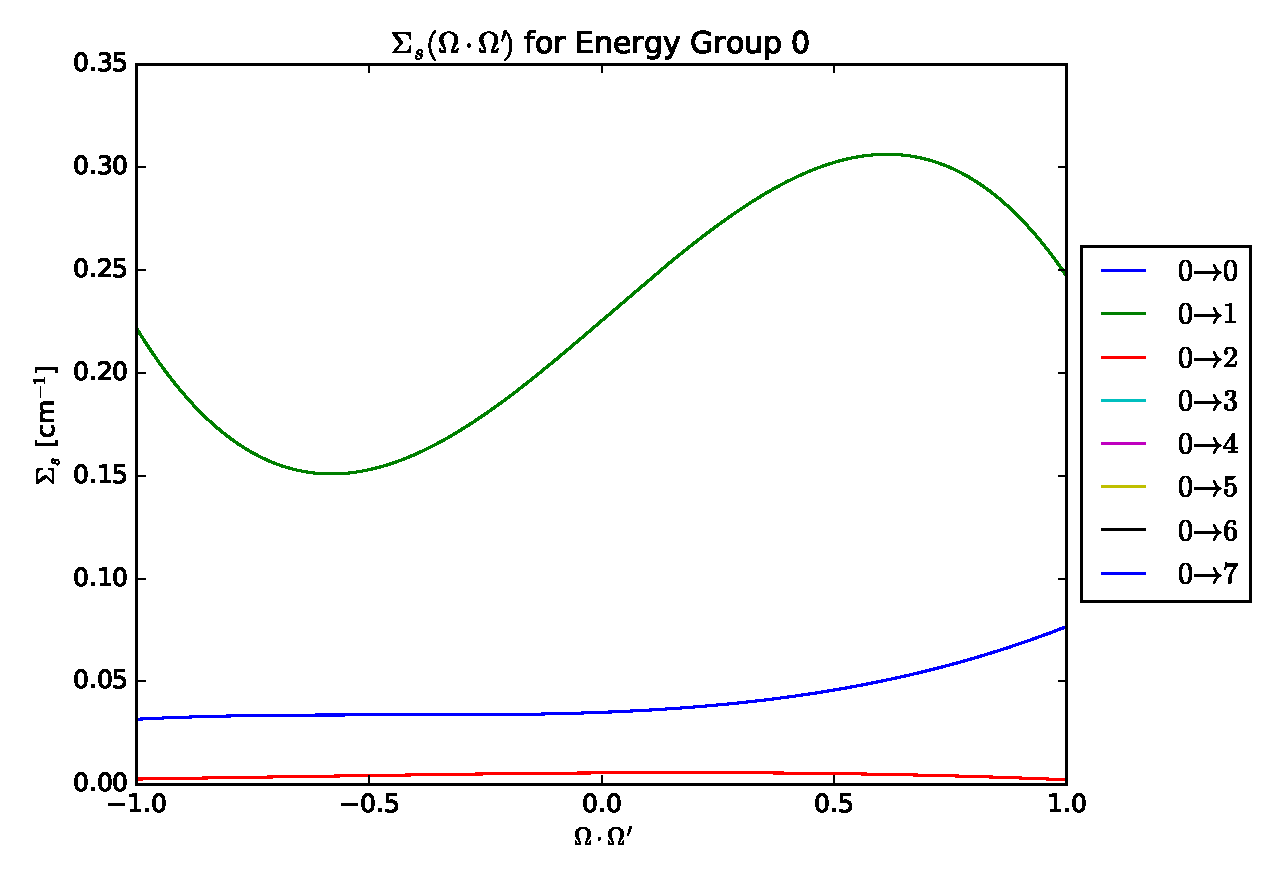
\includegraphics[width=\textwidth]{img/xs.eps}
\caption{Water scattering cross section as a function of angle in the highest energy group.}
\label{fig:water-xs}
\end{figure}
\FloatBarrier

In Figure \ref{fig:water-xs-coarse} we see that the coarse QR and LDO quadrature
sets both capture the forward-peakedness of this cross section. The QR quadrature set
contains fewer unique values of $\bo\cdot\bo'$ than does the LDO quadrature set,
however, and the LDO quadrature set produces values of $\Sigma_s$ that are closer to
the extremal values of the reference cross section curve. The potential impact of this
is the possibility of being able to use relatively coarse LDO quadrature sets in 
solving a problem while incorporating the problem's angular dependence better than a 
standard quadrature set of a similar coarseness would.

\begin{figure}[!htb]
\centering
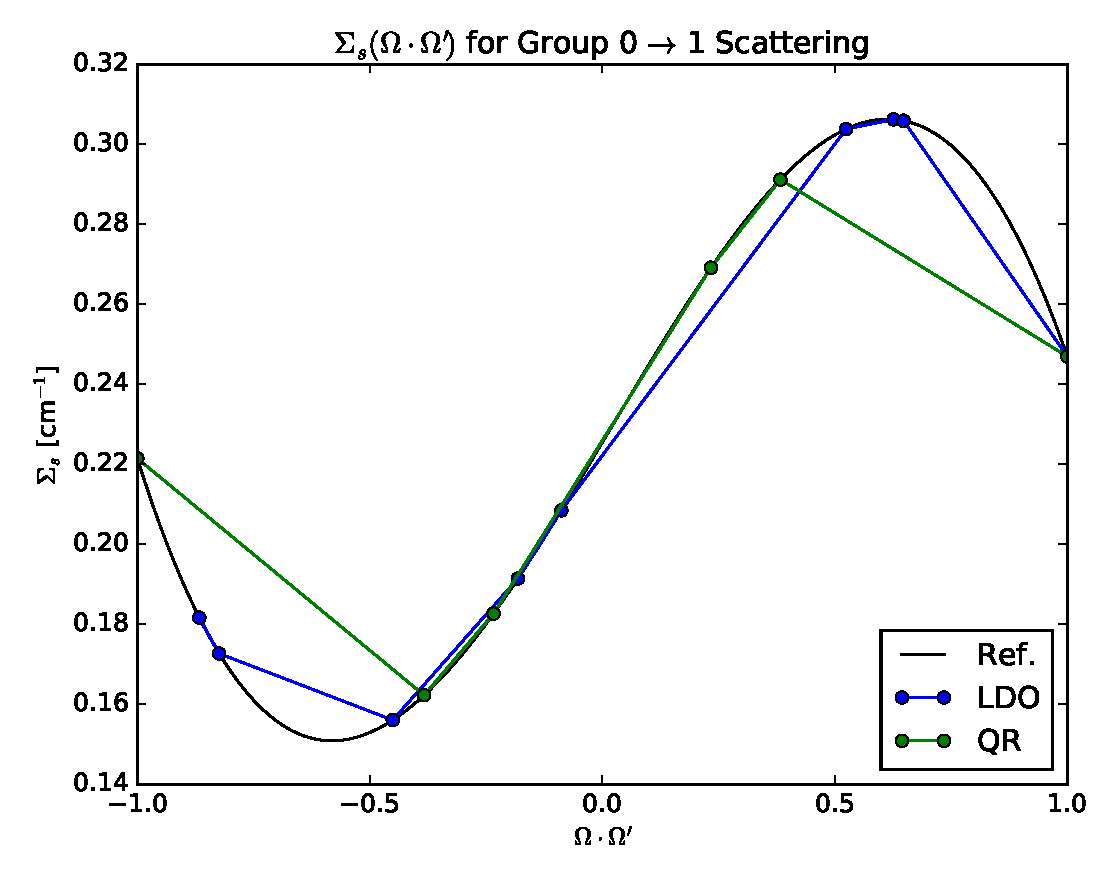
\includegraphics[width=\textwidth]{img/xs-coarse.eps}
\caption{Group 0 $\to$ 1 scattering cross section reconstructed with coarse angular meshes.}
\label{fig:water-xs-coarse}
\end{figure}
\FloatBarrier

Finer angular meshes of both quadrature set types are shown in Figure 
\ref{fig:water-xs-fine}; in this plot the QR quadrature set has 128 angles and the LDO 
quadrature set has 144 angles.
It is seen that both quadrature set types match the reference
cross section curve quite well when the angular mesh is refined. This is unsurprising
for the QR quadrature set and serves as a confirmation that the LDO formulation is 
formally the same as the traditional discrete ordinates equations.

\begin{figure}[!htb]
\centering
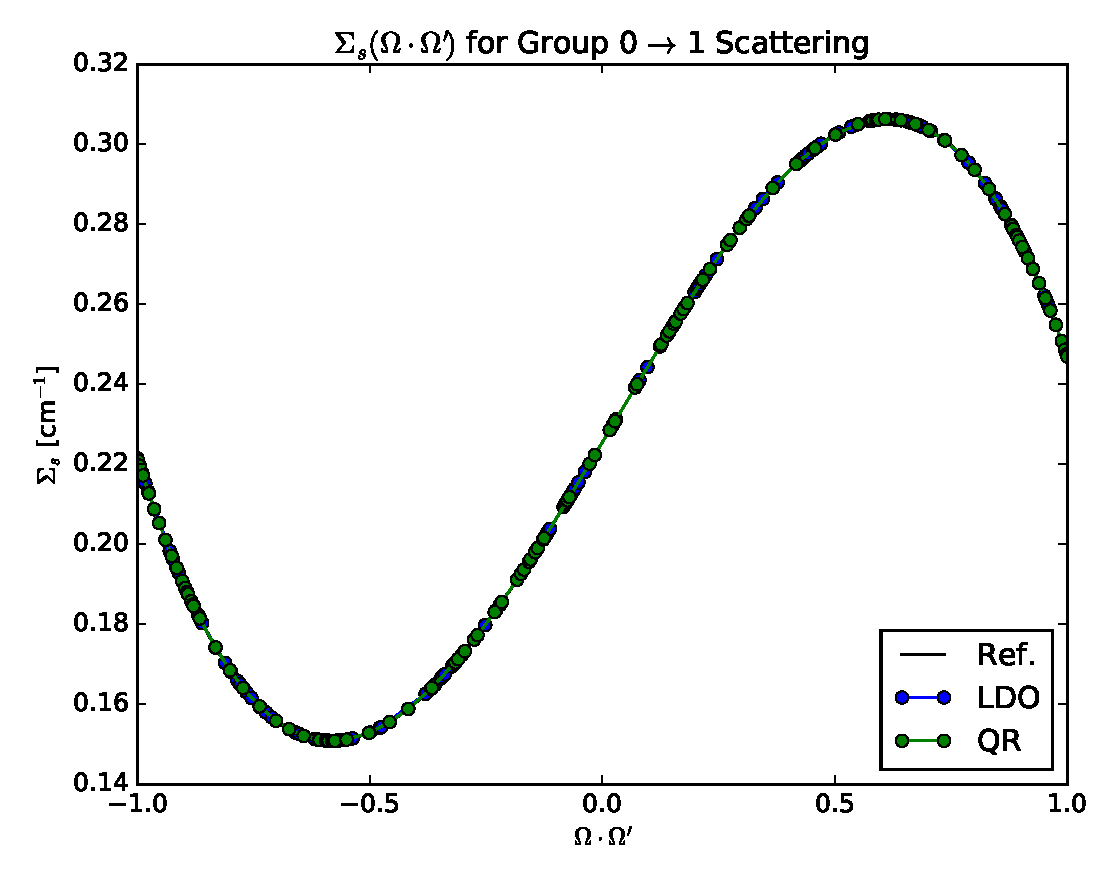
\includegraphics[width=\textwidth]{img/xs-fine.eps}
\caption{Group 0 $\to$ 1 scattering cross section reconstructed with fine angular meshes.}
\label{fig:water-xs-fine}
\end{figure}
% \FloatBarrier

\FloatBarrier
\subsection{Scattering in Denovo}

In Denovo and most other discrete ordinates codes, the operation $\mathbf{L}^{-1}$ in 
Equation \ref{l_inv} represents a sweep through the system mesh in the directions of 
particle travel \cite{denovo}. 
We can rewrite Equation \ref{l_inv} to reframe it as solving for the total source $Q$:

% eq 5 in the sweep sources pdf
\begin{equation}
Q = \ve{DL}^{-1}\left(\ve{M}Q_m + Q_d\right).
\label{swpsrc}
\end{equation}

\noindent Here, the operators are the same as those in Equation \ref{l_inv}, $Q_m$ is 
the sum of the ``moment-based'' sources, and $Q_d$ is the sum of the ``discrete'' 
sources \cite{sweepsources} as shown in Equation \ref{qmd}. Recalling Equation 
\ref{swpsrc}, moment-based sources are those to which the moment-to-discrete operator 
$\ve{M}$ is applied in the traditional discrete ordinates formulation. Discrete sources
are not operated on by $\ve{M}$ and may be restricted to a subset of the discrete 
angles used in a given problem.

\begin{equation}
Q_m = \sum_{s=1}^{S_m}Q_{m,s} \quad\text{ and }\quad Q_d = \sum_{s=1}^{S_d}Q_{d,s},
\label{qmd}
\end{equation}

\noindent where $Q_{m,s}$ is a particular moment-based sweep source, $Q_{d,s}$ is a
particular discrete-based sweep source, $S_m$ is the total number of moment-based 
sources in the system, and $S_d$ is the total number of discrete sources
\cite{sweepsources}. Figure \ref{swpsrclist} shows the sweep source hierarchy
implemented in Denovo, where the goal of the infrastructure is to calculate the total
source listed in Equation \ref{swpsrc} by performing a transport sweep over the 
combined particle sources.

\begin{figure}[!htb]
\centering
\includegraphics[width=\textwidth]{img/swp-src.png}
\caption{Sweep source hierarchy in Denovo \cite{sweepsources}.}
\label{swpsrclist}
\end{figure}

From this diagram, it is apparent that all scattering derives from a common base class,
the scattering sweep source base, and that this base class derives from the 
moment-based sweep source class.
The types of scattering supported include downscattering, within-group scattering,
upscattering, and first-collision scattering. The scattering classes share a great deal
of functionality, hence the implementation of the common base class. Because the
scattering sweep source is a type 
of moment-based sweep source, we note the particular difference in the operator
forms of the discrete ordinates and LDO formulations and how that translates into 
implementing scattering calculations in Denovo.

In the LDO formulation, the interpolation matrix $\mathbf{J}$ is applied to the 
moment-based sources. Looking at Equations \ref{l_inv} and 
\ref{ldo_op}, it is apparent that the operator order is different between the 
traditional discrete ordinates formulation and the LDO formulation, Namely, the product
of the scattering matrix and the moment-to-discrete or interpolation matrix is reversed
between the two sets of equations. To handle this difference, a ``scattering 
calculator'' was implemented in the scattering sweep source base class such that the
scattering sweep source is calculated in accordance with the formulation of the
equation set being solved.

\section{Selection of Quadrature Sets}

As mentioned in Section \ref{sec:ldo_math}, the LDO equations are developed with and
must be evaluated at a fundamental system of points for the subspace of spherical
harmonics. Ahrens provides references for examples of construction methods of these
point systems \cite{ahrens}. Like Ahrens, we have chosen to use the extremal point sets
developed and distributed by Womersley \cite{wom}.

Womersley's extremal systems are generated such that the associated Gram matrix is
positive definite \cite{wom}; these matrices are of interest to work with from an
implementation standpoint because of their low condition numbers. In Table \ref{md03}
we give an example of a point set generated by Womersley. The point set is of degree 3
and thus contains 16 points.

\begin{table}[!htb]
\centering
\caption{The ``md003.00016'' quadrature set developed by Womersley \cite{wom}.}
\small
\begin{tabular}{cccc}
\multicolumn{1}{c}{\textbf{$\mu$}} & 
\multicolumn{1}{c}{\textbf{$\eta$}} & 
\multicolumn{1}{c}{\textbf{$\xi$}} & 
\multicolumn{1}{c}{\textbf{$w$}} \\
\hline
0.00000000000000000 & 0.0000000000000000 & 1.0000000000000000 &
0.73999377643692810 \\
0.89273429807179527 & 0.0000000000000000 & -0.45058348066286125 &
0.73999377643692787 \\
-0.14301510478336188 & 0.98579910306911467 & -0.088015954189755163 &
0.73999377643692688 \\
-0.73214276086495222 & 0.51082433836573149 & -0.45058348066286003 &
0.73999377643692854 \\
0.65748213697787805 & -0.7831172071742225 & -0.088015954189756496 &
0.73999377643692765 \\
-0.70626478165373330 & 0.4595590936077425 & 0.52407635945553088 &
0.92161132427900849 \\
-0.60670408850507063 & -0.4914548265981833 & 0.62661538904237324 &
0.73999377643692887 \\
-0.29492456926406690 & -0.9812320737717869 & -0.18150577463199227 &
0.92161132427900960 \\
0.21767572867043725 & -0.7831172071742269 & 0.62661538904237279 &
0.73999377643692787 \\
-0.51446703219451573 & -0.23748738235169115 & -0.82396809162048790 & 
0.73999377643692743 \\
0.85155965361038066 & -0.013788611344369470 & 0.52407635945553044 &
0.92161132427900860 \\
0.28603020956672459 & -0.48914548265981850 & -0.82396809162048790 &
0.73999377643692776 \\
0.14962969730741976 & 0.47595590936077353 & -0.86664694427906974 &
0.92161132427900883 \\
-0.96739492195887000 & -0.23748738235169184 & -0.088015954189756274 & 
0.73999377643692821 \\
0.68136471239214502 & 0.72663286501151070 & -0.088015954189756274 &
0.73999377643692898 \\
0.22843682262779150 & 0.72663286501151014 & 0.64793618324097579 &
0.73999377643692754
\end{tabular}
\label{md03}
\end{table}

We note that all of Womersley's extremal systems are generated such that the first
point in each set is situated along the $z$-axis. These systems are rotationally
invariant with respect to the maximization of the logarithm of the determinant of the 
associated Gram matrix, so the point sets may be rotated in space if this vector
placement is undesirable for a given scenario. The work presented and discussed in 
Chapter \ref{sec:results} uses the point sets posted by Womersley; exploration of using
rotated extremal point sets is a potential area of future work.

\section{Restrictions}

Several restrictions exist for solving the LDO equations in the Exnihilo framework as
well as employing the solutions in the ADVANTG software. Some of these restrictions are
a result of implementing the LDO equations in a framework designed to solve the
traditional discrete ordinates equations, while other restrictions are merely 
current limitations of the software pieces used in this work.

\subsection{Boundary Conditions}
\label{sec:bc}

Although it is mathematically possible to use reflective boundary conditions for the
LDO equations (given their interpolatory nature), the current implementations of the
various codes used in this work restrict the solutions to vacuum (black) boundary
conditions at the time of this writing. The primary reason for this is that the
ADVANTG software does not support the use of reflective boundary conditions, and the
LDO equations were implemented into the Exnihilo framework for the purpose of using 
the solutions in ADVANTG for Monte Carlo variance reduction parameter generation. To a
lesser extent, the Exnihilo framework was built with symmetric quadrature sets in mind,
and so the use of reflective boundary conditions with the LDO equations was considered
to be an effort beyond the scope of this work.

\subsection{Uncollided Flux}
\label{sec:uncflux}

The use of an ``analytic'' approximation of the uncollided flux source,
a method employed to reduce ray effects from point sources or other small sources
\cite{exum}, is not available when solving the LDO equations through Exnihilo. This
approximation is obtained in Denovo by solving the following equations for the group
uncollided flux moments for every mesh cell in the calculation domain:

\begin{equation}
\bo\cdot\nabla\psi^g(\bo) + \sigt^g\psi^g(\bo) = \frac{Q^g_p}{4\pi}\delta(r-r_p),
\label{uncflux_eq}
\end{equation}

\noindent where $|r-r_p|$ is the geometric distance between the flux source and some
particular point and the analytic solution of the above equations is

\begin{equation}
\psi^g(\bo) = \delta(\bo - \bo_{p\rightarrow r})\frac{Q^g_p}{4\pi|r-r_p|^2}
e^{-\tau(r,r_p)}.
\label{uncflux_sln}
\end{equation}

\noindent In Equation \ref{uncflux_sln}, the term $\delta(\bo - \bo_{p\rightarrow r})$
indicates that the angular flux at a given point is only nonzero for the the angle that
passes directly from the source through the particular point of interest. The ``optical
path length'' $\tau(r,r_p)$ is the integral of the total cross section from the 
source location to the point of interest and is calculated via ray tracing.

Because the Exnihilo framework was written to solve the traditional form of 
the discrete ordinates equations, these flux moment solutions in Equation
\ref{uncflux_sln} are based on the expansion listed in Equation \ref{sph_harm_exp}.
That is to say, when using the analytic uncollided flux approximation, the flux moments
are calculated using the components of the spherical harmonic functions listed in
Equations \ref{eq:sph_e} and \ref{eq:sph_o}. So, the solutions do not apply to the LDO
equations and this treatment cannot be used. All tests in the following chapter were
run with the uncollided flux treatment turned off; implementing this approximation for
use with the LDO equations in Denovo remains an area of future work.

\subsection{Particle Sources}
\label{sec:ptsrc}

When considering neutron transport problems of interest, a small variety of particle 
source types appear frequently. One typical source type is an isotropic source, in 
which particles are emitted uniformly in all directions. Specifically, isotropic point 
sources, in which the physical size of the source itself is negligible, are routinely 
used in both experimental work and simulations.

Point sources must be approximated as small volumetric sources when solving the LDO
equations in Denovo. When a point source is used in a system, Denovo calculates the
uncollided flux from that point source using the analytic solution to the NTE. As
mentioned previously, this is done to alleviate ray effects. However, as discussed 
above in Section \ref{sec:uncflux}, these analytic solutions are not applicable when
solving the LDO equations. Thus, when a point source is specified in combination with 
the LDO equations, it is treated as a small volume source instead. In this case, an
equal contribution of the source strength is added to every angular flux coefficient in
the cell in which the particle source resides. This is notably different from the
traditional discrete ordinates formulation in Denovo, in which the source strength is
added only to the zeroth flux moment for reasons described in Section \ref{sec:flux}.

Finally in this section, we note that this work is limited to isotropic particle
sources. At the time of this writing, ADVANTG does not support directional sources 
\cite{munk}; Monte Carlo particle importance maps generated with ADVANTG and Denovo
automatically use an isotropic source distribution regardless of the particle source
input. Since the ultimate goal of implementing the LDO equations in the Exnihilo
framework is to use the results for Monte Carlo variance reduction parameter 
generation via ADVANTG, implementation of the use of directional sources when solving 
the LDO equations in Denovo was not pursued in this work.

\subsection{Fixed Source vs. Criticality Calculations}

All scenarios tested in this work are fixed-source problems, though the LDO equations
are applicable to $k$-eigenvalue (criticality) problems in principle. Ray effects,
which we are interested in using solutions of the LDO equations to mitigate, largely
come from localized sources, as discussed in Section \ref{sec:ray}. Due to the 
distributed nature of fission sites in a typical light water reactor, the particle 
flux in a given criticality calculation will be relatively isotropic and unlikely to 
incur ray effects within the reactor core. Furthermore, at the time of this writing, 
ADVANTG only supports generation of Denovo input for fixed-source problems. 
